\section{Design Overview}
\label{s:design}
%
\begin{figure}[t]
\centering
    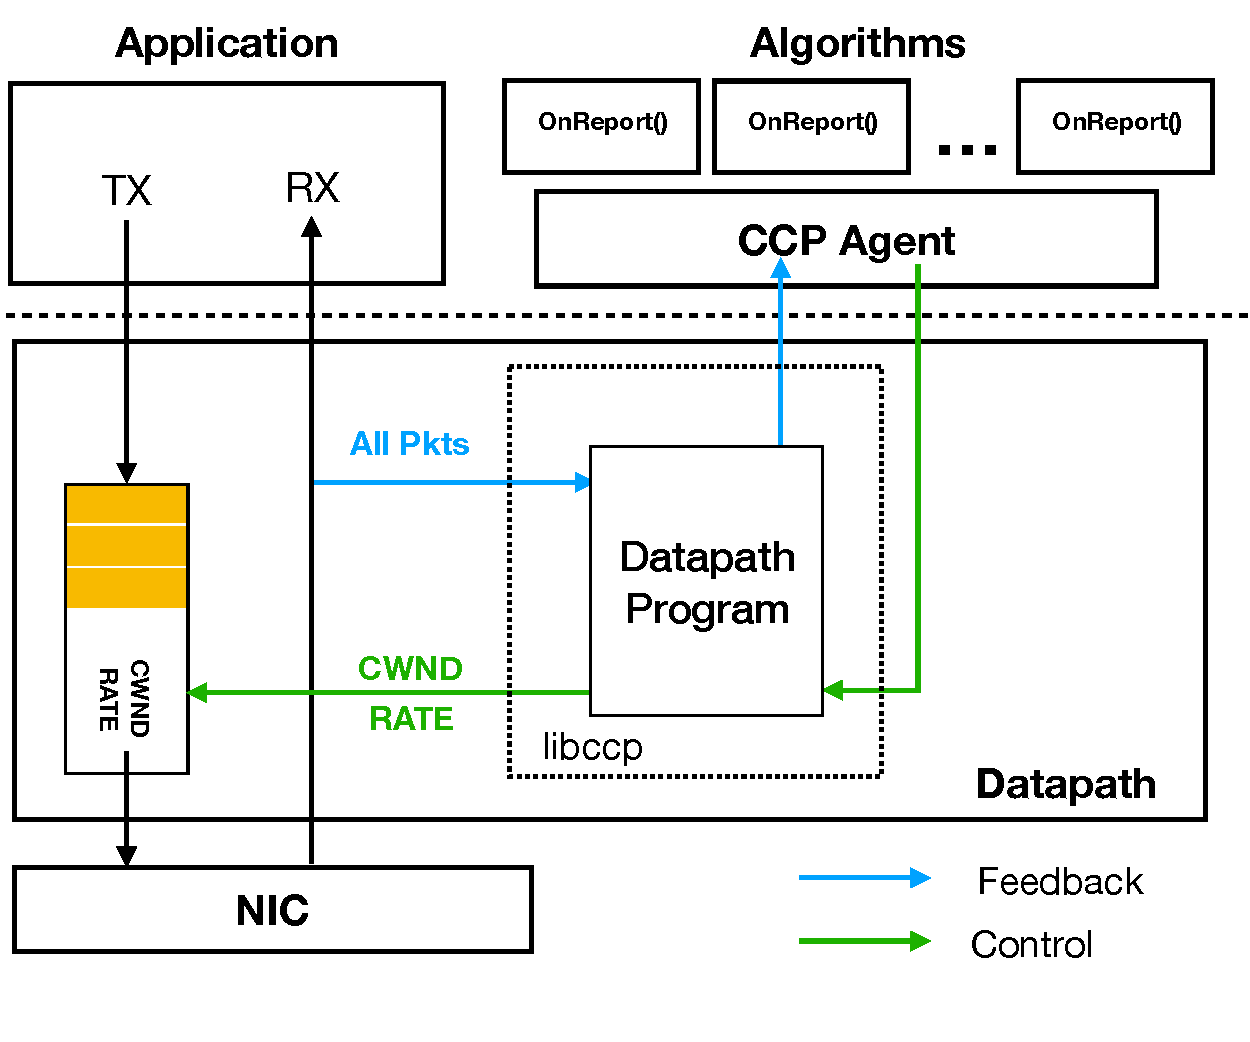
\includegraphics[width=\columnwidth]{img/ccp_design_sigcomm}
    \caption{Congestion control algorithms in CCP are distinct from the application and datapath.
    Users specify control patterns to set the congestion window or rate,
    and fold functions to define how to summarize datapath messages into reports processed in CCP.}\label{fig:design}
\end{figure}
%
Our design restructures congestion control by separating it into two distinct components: an off-datapath agent (CCP) and a set of interfaces that the datapath must provide. The CCP agent provides the execution environment for user-specified congestion control algorithms. It receives data about congestion signals from the datapath and invokes the algorithm's code that uses this data. The datapath is responsible for processing feedback (e.g., TCP or QUIC ACKs) from the receiver to provide congestion signals for the algorithms that run in CCP. The datapath also provides interfaces for CCP algorithms to set the congestion window and pacing rate, and express control patterns; these patterns can control transmission times and specify the times at which congestion signals are delivered to CCP.

\subsection{CCP Design Principles}
\label{s:datapath:isolation}

To enable rich new congestion control algorithms on the Linux networking stack,
CCP must provide a low-barrier programming environment and access
to libraries (\eg for optimization, machine learning, \etc).
%
Further, new algorithms should also achieve high performance running at tens of
Gbit/s per connection with small ``in-stack'' packet delays.

However, supporting experimentation and libraries (typically
\userspace code) means that congestion control algorithm code is untrusted.
Otherwise, bugs in algorithm or library code could cause kernel
crashes or create vulnerabilities that could trigger privilege escalation
attacks on the kernel.

\Para{Explicit fast and slow path separation.} While algorithms must have
some component running in the same address space as the kernel to collect measurements,
we restrict this functionality by requiring {\em explicit fast and slow path} components for algorithms:
the fast path runs in the Linux kernel, and the slow path in \userspace.
%
An alternative, which is to allow fully functional kernel modules with software
fault isolation (\eg LXFI~\cite{lxfi}) from the rest of the kernel, will likely
involve significant performance impediments.\footnote{Further, an approach such as
LXFI also requires a careful annotation of kernel functions, and the
specification of principals and kernel API integrity rules---a challenging
task because the network stack has a large number of functions with subtle
behaviors.}
%
Instead, our fast path programs are written in a restrictive domain-specific language (\Sec{sec:ccp})
that is free from broad classes of vulnerabilities.\footnote{Note that while \texttt{libccp}, our fast path library (\Sec{s:datapath:libccp}), enforces runtime safety of fast-path algorithm logic,
algorithm implementations are nevertheless free to set arbitrary rates or congestion windows.
As any application can open UDP sockets and congest the network, we do not restrict this behavior.}
Meanwhile, slow path programs have full access to the \userspace programming environment,
tools, and libraries.

Explicit fast and slow path separation also enables future use cases where the
slow paths of algorithms may run on a machine different from the sender to
centralize congestion control policies across groups of hosts.

\an{introduce terminology: fold function, control pattern, etc}

\begin{table}[]
    \centering
    \begin{tabular}{c|c|c}
        Implementation & Reporting Interval & Mean Throughput \\
        \hline
        Kernel & - & $43$ Gbit/s \\
        CCP & Per ACK & $29$ Gbit/s \\
        CCP & Per $10$ ms & $41$ Gbit/s \\
    \end{tabular}
    \caption{Single-flow throughput for different reporting intervals between
      the Linux kernel and CCP \userspace, compared to kernel TCP
      throughput. Per-ACK feedback (0 $\mu$s interval) reduces throughput by
      32\% while using a $10$ ms reporting interval
      achieves almost identical throughput to the kernel. Results as the number
      of flows  increases are in
      \S\ref{sec:eval:whyfold}.}\label{tab:perf:interval}
\end{table}

\Para{Decoupling algorithm logic from the ACK clock.} Typical congestion control
implementations in the Linux kernel are coupled to the so-called ``ACK-clock,''
\ie algorithm functionality is invoked upon receiving a packet acknowledgment in
the networking stack.
%
While this is also true of a CCP algorithm's fast path, the CCP slow path is
only invoked when the user specifies, whether less frequently than per-ACK or in response to certain urgent conditions.
%
To support this, CCP exposes a \ct{report} instruction for fast path programs to send a
report of the most recent user-defined measurement state in the kernel to the slow path.

This decoupling of algorithm logic from the ACK clock has two benefits.
%
First, the user can develop congestion control algorithms free from the strict
time restrictions rooted in the inter-arrival time of packet acknowledgments,
especially at high link rates.
Hence, users can implement algorithms that use complex logic and yet retain high performance.

Second, providing per-ACK notifications from the kernel to \userspace would incur
significant overhead.
%
Table~\ref{tab:perf:interval} shows that for a single saturating \ct{iperf}
connection over a loopback interface, Linux kernel TCP on a server machine
with four 2.8-Ghz cores achieves $45$ Gbit/s running Reno.
%
In comparison, per-ACK reporting from the kernel to the CCP \userspace achieves
only 68\% of the kernel's throughput.
%
By increasing the time between reports sent to the slow path to 10 ms (see the
``per 10 ms'' row), CCP Reno achieves close to the kernel's throughput.

Given that CCP should report measurements only infrequently, a key question is
how best to summarize congestion signals within the fast path, so that CCP
algorithms can achieve high fidelity compared to a baseline that implements the
algorithm completely within the kernel.
Although we are optimistic that a good design can achieve high fidelity because the natural time-scale for end-to-end
congestion control is the RTT between sender and receiver,
achieving it requires a careful design of the information channel between the kernel and CCP \userspace.
Indeed, in \S\ref{sec:eval:fidelity} we show that using a
larger reporting period does not affect the fidelity of CCP algorithm
implementations relative to native in-kernel implementations.

\subsection{Alternate Designs}
\label{sec:design:alternatives}

\an{eBPF is limited and pluggable tcp is strictly less general than us.}

\an{address congestion manager here}

\subsection{CCP-Datapath Isolation}

Should CCP run in the same address space as the datapath or not? There are some trade-offs involved in this decision. On the plus side, if run in the same address space, then information could be exchanged between them nearly instantaneously at high bandwidth, and a congestion signal could be sent from the datapath to CCP every time feedback from the receiver arrives. But there are two drawbacks to this approach:

\paragrapha{Safety} Bugs in CCP or in the algorithm's code could cause datapath crashes, or cause vulnerabilities that trigger privilege escalation attacks on kernel datapaths. 
To cope, at a minimum, we would have to enforce restrictions on the kernel functions that CCP can use, and adopt methods from recent research on kernel software fault isolation (LXFI~\cite{lxfi}). 
This approach will have a non-trivial performance impact, quite likely defeating the purpose of running CCP in the same address space as the datapath. 
This approach also requires a careful annotation of kernel functions, and the specification of principals and kernel API integrity rules, a challenging task because the network stack has a large number of functions with subtle behaviors.
    
\paragrapha{Flexibility} In the future, we anticipate running CCP on a different machine from the sender to centralize congestion control policies across groups of hosts. 
The same-address-space CCP would require a substantial re-design for this mode of operation.

\begin{table}[]
    \centering
    \begin{tabular}{c|c|c}
        Implementation & Reporting Interval & Mean Throughput \\
        \hline
        Kernel & - & $43$ Gbit/s \\
        CCP & Per ACK & $29$ Gbit/s \\
        CCP & Per $10$ ms & $41$ Gbit/s \\
    \end{tabular}
    \caption{Single-flow throughput for different reporting intervals between the Linux TCP datapath and user-space CCP, compared to kernel TCP throughput. Per-ACK feedback (0 $\mu$s interval) reduces throughput by 32\%, a significant amount, while using a $10$ ms reporting interval achieves almost identical throughput to the kernel. Results as the number of flows  increases are in \S\ref{sec:eval:whyfold}.}\label{fig:perf:interval}
\end{table}

\smallskip

Our design supports both modes, but we focus on how to achieve high performance and fidelity when CCP is in a different address space, including the important case when the datapath is kernel TCP and CCP is in user space.

When CCP is in a different address space, providing per-ACK notifications from the datapath to CCP incurs high overhead, as shown in Figure~\ref{fig:perf:interval}. This experiment shows that for a saturating iperf connection over a loopback interface, the Linux kernel TCP on this machine  (with 4 2.8 Ghz cores) achieves $45$ Gbit/s running Reno, whereas per-ACK reporting from the kernel datapath to CCP running Reno achieves only 68\% of the throughput of the kernel. 
One way to improve performance is to increase the time between reports sent to CCP. The ``Per 10 ms'' bar shows that a less frequent reporting period achieves close to the kernel's throughput. 
%\ma{are we going to add more reporting periods (other than 10 ms) to the figure?}

\if 0
One could combat this issue by moving CCP closer to the datapath; \ie either by placing them in the same address space or perhaps by using more efficient IPC mechanisms. Indeed, the design of CCP allows for such solutions. 

\fi

Given that CCP should report measurements only infrequently, a key question is how best to {\em summarize} congestion signals on the datapath so that CCP algorithms can achieve high fidelity compared to a baseline that implements the algorithm within the datapath. 
Although we are optimistic that a good design can achieve high fidelity because the natural time-scale for end-to-end congestion control is the RTT between sender and receiver, achieving it requires a careful design of the information channel between datapath and CCP. 

In \S\ref{sec:eval:fidelity} we show that using a larger reporting period does not affect the fidelity of CCP algorithm implementations relative to native datapath ones. 
